\documentclass[14pt]{beamer}
\usetheme{defense}
\graphicspath{{../../figures/}}


\usepackage[final]{listofsymbols}
\usepackage{tikz}
\usepackage{svg}
\usepackage{anyfontsize}
\opensymdef
\newsym[Pointwise multiplication operator]{omult}{\odot}
\newsym[Unit vector, containing only ones]{vunit}{\overrightarrow{1}}

\newsym[Area]{symA}{A}
\newsym[Neural Network bias vector]{symvb}{\overrightarrow{b}}
\newsym[LSTM cell state vector]{symvc}{\overrightarrow{c}}
\newsym[Electrical capacitance]{symC}{C}
\newsym[LSTM candidate cell state vector]{symvct}{\overrightarrow{cc}}
\newsym[LSTM forget gate vector]{symvf}{\overrightarrow{f}}
\newsym[Electrical conductance]{symG}{G}
\newsym[Recurrent Neural Network hidden state vector]{symvh}{\overrightarrow{h}}
\newsym[GRU candidate hidden state vector]{symvhh}{\overrightarrow{ch}}
\newsym[Neural Network hidden perceptron]{symH}{H}
\newsym[Electrical current]{symi}{i}
\newsym[LSTM input gate vector]{symvi}{\overrightarrow{i}}
\newsym[Neural Network input perceptron]{symI}{I}
\newsym[Electrical inductance]{symL}{L}
\newsym[Memristor's internal resistance, memristance]{symM}{M}
\newsym[LSTM output gate vector]{symvo}{\overrightarrow{o}}
\newsym[Neural Network output perceptron]{symO}{O}
\newsym[LSTM peephole weight vector]{symvp}{\overrightarrow{p}}
\newsym[Electrical charge]{symq}{q}
\newsym[GRU reset gate vector]{symvr}{\overrightarrow{r}}
\newsym[Electrical resistance]{symR}{R}
\newsym[Time]{symt}{t}
\newsym[Electrical voltage]{symv}{v}
\newsym[Neural Network weight]{symw}{w}
\newsym[Neural Network weight matrix]{symmw}{\mathit{W}}
\newsym[Neural Network input vector]{symvx}{\overrightarrow{x}}
\newsym[GRU update gate vector]{symvz}{\overrightarrow{z}}
\newsym[Electrical flux]{symphi}{\phi}
\newsym[Memristor's internal conductance, memductance]{symW}{\kappa}
\closesymdef
\markasused{omult}


\setcounter{tocdepth}{1}

\newcommand<>{\overlay}[1]{\only#2{%
  \AddToHookNext{shipout/foreground}{%
    \begin{tikzpicture}[overlay]%
      \draw[fill=black,opacity=0.70]
      (current page.north east) rectangle (current page.south west);
      \node at (current page.center) {#1};
    \end{tikzpicture}}}
    }

    \title{Memristors-based recurent modules for neural computing}

    \newcommand {\Supervisor} {
      {Dr. Diogo Caetano} and {Dr. Ruxandra Barbulescu}}
    \newcommand {\CommitteeMembers} {
      {Dr. Frédéric Pétrot}}
    \newcommand {\Chairperson} {{Dr. Florence Maraninchi}}
    \author[V. BARBAZA]{{Valentin BARBAZA}}

    \date{17 november 2023}

    \logo{
      \begin{tikzpicture}[overlay,remember picture]
        \node[left=0cm] at (current page.33){
          
\includegraphics[height=1cm]{logos/inesc-mn.png}
          \hspace{1pt}
          
\includegraphics[height=1cm]{logos/ist.eps}
          
\includegraphics[height=1cm]{logos/inesc-id.eps}
        };
      \end{tikzpicture}
    }

    \begin{document}

    \frame{\titlepage}

    \begin{frame}
      \frametitle{Table of Contents}
      \tableofcontents
    \end{frame}

    \section{Motivation and objectives}

    \begin{frame}{\insertsection}
      \begin{columns}
        \column{.6\textwidth}
        \begin{itemize}
          \item NNs complexity grows rapidly
        \end{itemize}
        \vspace{0.5cm}
        \begin{equation*}\label{eq:nnHid}
          \footnotesize
          \begin{bmatrix}
            H_1\\ H_2\\ H_3\\ H_4\\
          \end{bmatrix}
          =
          \begin{bmatrix}
            w_h_{1,1} & w_h_{1,2} & w_h_{1,3}\\
            w_h_{2,1} & w_h_{2,2} & w_h_{2,3}\\
            w_h_{3,1} & w_h_{3,2} & w_h_{3,3}\\
            w_h_{4,1} & w_h_{4,2} & w_h_{4,3}\\
          \end{bmatrix}
          \cdot
          \begin{bmatrix}
            I_1\\ I_2\\ I_3\\
          \end{bmatrix}
        \end{equation*}
        \column{.4\textwidth}
        \includesvg[width=\columnwidth,pretex=\scriptsize]{NN_explained.svg}
      \end{columns}
    \end{frame}

    \begin{frame}{\insertsection}
      \begin{columns}
        \column{.6\textwidth}
        \begin{itemize}
          \item Reduce computation time by using analog
          \item Allows use for time sensitive problems
        \end{itemize}
        \column{.4\textwidth}
        \includesvg[width=\columnwidth,pretex=\scriptsize]{NN_explained.svg}
      \end{columns}
    \end{frame}

    \section{Introduction}

    \begin{frame}{\insertsection}{RNNs}
      \begin{columns}
        \column{.6\textwidth}
        RNNs are a type of NN :
        \begin{itemize}
          \item Used for time dependent data
          \item That have a feedback connection
        \end{itemize}
        \column{.4\textwidth}
        \includesvg[width=.8\columnwidth,pretex=\small]{rnn/rnnFolded}
      \end{columns}
      \vspace{0.8cm}

      \begin{equation*}\label{eq:rnn}
        \overrightarrow{h_t}=f(\overrightarrow{x_t},\overrightarrow{h_{t-1}})
      \end{equation*}
    \end{frame}

    \subsection{LSTMs}

    \begin{frame}{\insertsection}{\insertsubsection}
      \includesvg[width=\columnwidth,pretex=\scriptsize]{lstm/lstmCell}
    \end{frame}

    \begin{frame}{\insertsection}{\insertsubsection}
      \begin{columns}
        \column{.4\textwidth}
        \begin{itemize}
          \item<1-> Sigmoid and a VMM
          \item<2-> tanh and a VMM
          \item<3-> Pointwise multiplications
        \end{itemize}
        \column{.6\textwidth}
        \only<1->{\begin{equation*}\label{eq:inputG}
          \overrightarrow{i_t}=\sigma ([\overrightarrow{x_{t}},\overrightarrow{h_{t-1}}]\cdot w_i + \overrightarrow{b_i})
        \end{equation*}
        \begin{equation*}\label{eq:forgetG}
          \overrightarrow{f_t}=\sigma ([\overrightarrow{x_{t}},\overrightarrow{h_{t-1}}]\cdot w_f + \overrightarrow{b_f})
        \end{equation*}
        \begin{equation*}\label{eq:outputG}
          \overrightarrow{o_t}=\sigma ([\overrightarrow{x_{t}},\overrightarrow{h_{t-1}}]\cdot w_o + \overrightarrow{b_o})
        \end{equation*}}
        \only<2->{\begin{equation*}\label{eq:candCell}
          \overrightarrow{\tilde{c}_t}=tanh([\overrightarrow{x_{t}},\overrightarrow{h_{t-1}}]\cdot w_c+ \overrightarrow{b_c})
        \end{equation*}}
        \only<3->{\begin{equation*}\label{eq:cellS}
          \overrightarrow{c_t}=\overrightarrow{f_t}\odot \overrightarrow{c_{t-1}} + \overrightarrow{i_t} \odot \overrightarrow{\tilde{c}_t}
        \end{equation*}
        \begin{equation*}\label{eq:hiddenS}
          \overrightarrow{h_t}=\overrightarrow{o_t}\odot tanh(\overrightarrow{c_t})
        \end{equation*}
        }
      \end{columns}
    \end{frame}


    \begin{frame}{\insertsection}{Memristors}
      \begin{columns}
        \column{.65\textwidth}
        \includesvg[width=\columnwidth,pretex=\tiny]{memristor/memristor}
        \column{.4\textwidth}
        \begin{itemize}
          \item Recent electrical component
          \item Variable resistance
        \end{itemize}
      \end{columns}
    \end{frame}


    \section{The circuits}

    \begin{frame}<1>[label=frme:lstm]
      \frametitle{\insertsection}
      \begin{center}
        \begin{tikzpicture}[overlay]
          \node at (4, 1){
            \includesvg[width=3cm,pretex=\fontsize{4}{5}\selectfont]{lstm/lstmCell}
          };
        \end{tikzpicture}
        \begin{tikzpicture}
          \node[anchor = south west, inner sep = 0] (image) {        \includesvg[width=1\columnwidth,pretex=\fontsize{4}{5}\selectfont]{lstm/lstmCircuit}};
          \begin{scope}[shift={(image.south west)},x={(image.south east)},y={(image.north west)}]

            \draw<2>[red,thick,rounded corners] {(0.13,0.84) rectangle (0.21,0.76)};
            \draw<2>[red,thick,rounded corners] {(0.65,0.84) rectangle (0.72,0.76)};
            \draw<3>[red,thick,rounded corners] {(0.03,0.62) rectangle (0.10,0.54)};
            \draw<4>[red,thick,rounded corners] {(0.02,1) rectangle (0.20,0.85)};
          \end{scope}

        \end{tikzpicture}

      \end{center}
    \end{frame}

    \againframe<2>{frme:lstm}

    \subsection{Activation functions}
    \begin{frame}{\insertsection}{\insertsubsection}
      \begin{columns}
        \column{.7\textwidth}
        \includesvg[width=\columnwidth,pretex=\scriptsize]{activation/afCircuit}
        \column{.4\textwidth}
        \begin{itemize}
          \item Creates analog activation functions
          \item Is used for both tanh and sigmoid activation functions
        \end{itemize}
      \end{columns}
    \end{frame}

    \begin{frame}{\insertsection}{\insertsubsection}
      \begin{center}
        \includesvg[width=0.75\columnwidth,pretex=\tiny]{activation/afGraph}
      \end{center}
    \end{frame}

    \subsection{Memory cell}
    \againframe<3>{frme:lstm}

    \begin{frame}{\insertsection}{\insertsubsection}
      \begin{columns}
        \column{.65\textwidth}
        \includesvg[width=\columnwidth,pretex=\tiny]{memcell/memCircuit}
        \column{.4\textwidth}
        \begin{itemize}
          \item Stores analog value
          \item Has two CMOS switches to avoid leakage
        \end{itemize}
      \end{columns}
    \end{frame}

    \begin{frame}{\insertsection}{\insertsubsection}
      \begin{center}
        \includesvg[width=.75\columnwidth,pretex=\tiny]{memcell/data-loss}
      \end{center}
    \end{frame}

    \subsection{Crossbar circuit}
    \againframe<4>{frme:lstm}

    \begin{frame}{\insertsection}{\insertsubsection}
      \begin{columns}
        \column{.4\textwidth}
        \begin{itemize}
          \item Performs analog VMM
          \item Can be parallel or serialized
        \end{itemize}
        \column{.65\textwidth}
        \includesvg[width=\columnwidth, pretex=\tiny]{crossbar/crossbarUse}
      \end{columns}
    \end{frame}

    \begin{frame}{\insertsection}{\insertsubsection}
      \includesvg[width=\columnwidth, pretex=\tiny]{crossbar/doubleMem}
      \begin{equation*}
        \label{eq:doubleMem2}
        y_0=R_f\cdot\sum_{k=0}^n(\sigma_{k+}-\sigma_{k-})\cdot x_k
      \end{equation*}
    \end{frame}

    \section{The tools}
    \subsection{Weight generation}
    \begin{frame}{\insertsection}{\insertsubsection}
      The weights are trained :
      \hfill\includegraphics[width = 4cm]{tensorflowKeras.jpg}
      \begin{itemize}
        \item Using Keras framework implemented in tensorflow python module
        \item In software and exported to a file
        \item Using the analog activation functions
      \end{itemize}
    \end{frame}

    \subsection{Netlist generation}
    \begin{frame}{\insertsection}{\insertsubsection}
      I created a script capable of generating modular netlist. It can take in :
      \begin{itemize}
        \item Any number of inputs
        \item Any serial size
        \item Dense layers
        \item LSTM layers
        \item GRU layers (Experimental)
      \end{itemize}
    \end{frame}



    \section{Results}
    \subsection{Airline}

    \begin{frame}{\insertsection}{\insertsubsection}
      \only{The airline problem is a forecasting problem using the monthly number of passengers on international airlines from 1949 to 1960.}

      \begin{tikzpicture}
        \node[anchor = south west, inner sep = 0] (image) {\includesvg[width=\columnwidth,pretex=\tiny]{datasets/airline}};
        \begin{scope}[shift={(image.south west)},x={(image.south east)},y={(image.north west)}]
          \filldraw<2>[black,opacity=0.9,even odd rule,rounded corners] {(0.68,0.93) rectangle (0.99,0.1)};
        \end{scope}

      \end{tikzpicture}

    \end{frame}

    \begin{frame}{\insertsection}{\insertsubsection}
      \begin{columns}
        \column{.7\textwidth}
        \includesvg[width=\columnwidth,pretex=\tiny]{results/airline/digital}
        \column{.3\textwidth}

        RMSE : 52.3 thousands passengers
      \end{columns}
    \end{frame}

    \begin{frame}{\insertsection}{\insertsubsection}
      \begin{columns}
        \column{.66\textwidth}
        \includesvg[width=\columnwidth,pretex=\tiny]{results/airline/analog}
        \column{.4\textwidth}
        \scriptsize
        \begin{tabular}{|c|c|c|}
          \hline
          Predictions & RMSE & Inference\\
          & & time\\
          \hline
          Analog & & \\
          ($n_s=1$) & 28.4 & $\approx 2.4 ms$\\
          \hline
          Analog & & \\
          ($n_s=2$) & 92.6 & $\approx 4.7 ms$\\
          \hline
          Analog & & \\
          ($n_s=4$) & 68.5 & $\approx 9.2 ms$\\
          \hline
          Digital & 0 & $\approx 5 s$\\
          \hline
        \end{tabular}
      \end{columns}
    \end{frame}

    \subsection{C. elegans}
    \begin{frame}{\insertsection}{\insertsubsection}
      \begin{columns}
        \column{.35\textwidth}
        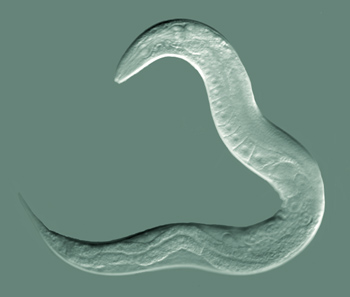
\includegraphics[height=15mm]{celegansPic.jpg}
        Regression problem with :
        \begin{itemize}
          \item 4 inputs
          \item 1000 time steps
          \item 40 sequences
        \end{itemize}
        \column{.7\textwidth}
        \includesvg[width=.95\columnwidth,pretex=\tiny]{datasets/celegans/ioValid0}
      \end{columns}
    \end{frame}

    \begin{frame}{\insertsection}{\insertsubsection}
      \begin{tikzpicture}
        \node[anchor = south west, inner sep = 0] (image) {\includesvg[width=\columnwidth,pretex=\tiny]{results/celegans/smooth5}};
        \begin{scope}[shift={(image.south west)},x={(image.south east)},y={(image.north west)}]
          \filldraw<2>[black,opacity=0.8,even odd rule,rounded corners] {(0.72,0.73) rectangle (0.99,0.31)};
          \draw<2>[red,thick,rounded corners] {(0.72,0.30) rectangle (0.99,0.16)};
        \end{scope}

      \end{tikzpicture}
    \end{frame}

    \begin{frame}{\insertsection}{\insertsubsection}
      \begin{columns}
        \column{.3\textwidth}
        \scriptsize
        RMSEs are :
        \begin{itemize}
          \item $0.073$ from analog to digital
          \item $0.066$ from analog to target
          \item $0.051$ from digital to target
        \end{itemize}
        Inference times are :
        \begin{itemize}
          \item $\approx 35s$ for digital
          \item $\approx 2.6s$ for analog
        \end{itemize}
        \column{.8\textwidth}
        \includesvg[width=\columnwidth,pretex=\tiny]{results/celegans/smooth5VB1}
      \end{columns}
    \end{frame}

    \section{Environmental and societal impact}
    \subsection{Environmental impact}

    \begin{frame}{\insertsection}{\insertsubsection}
      Chip frabrication :
      \begin{itemize}
        \item TMSC represent 5 \% of Taiwan's electrity consumption.
        \item Projected $86\cdot 10^9kg\, eq.\, CO_2$ by 2030.
      \end{itemize}
      Chip disposal.
    \end{frame}

    \subsection{Societal impact}

    \begin{frame}{\insertsection}{\insertsubsection}
      \begin{itemize}
        \item No RGPD to worry about.
        \item Increases digital divide.
      \end{itemize}
    \end{frame}

    \section{Conclusion}

    \begin{frame}{\insertsection}
      \begin{itemize}
        \item Full LSTM circuit simulation
        \item Verilog-A memristor model implementation
        \item Script that can generate modular netlists
        \item Ability to serialize or not the circuit
        \item Implementation of analog activation functions
        \item Experimental GRU capable circuit
      \end{itemize}
    \end{frame}

    \begin{frame}{\insertsection}
      \begin{itemize}
        \item Good results when running the circuit
        \item Significantly faster results
        \item Instability when dealing with large amount of time steps
      \end{itemize}
    \end{frame}

  \end{document}
